\section{Images as layers of fluorescence}
\label{imaging:model}


The goal of quantitative biological imaging, in overly general terms, is to perform
a set of meaningful mathematical operations on fluorescent images.
We therefore require a mathematical model of fluorescence images
to use as a reference when discussing image correction and analysis.
Note that the model I construct below is designed
to be intuitive with respect to cell culture microscopy,
and so it differs slightly from the
more general models that it is founded upon
\cite{Schultz1974,Madiset1998,L2000,Model2001}.


A fluorescence microscopy image $I$ can be thought of as
a series of fluorescing layers, each with its own distinct properties,
that add together to create the final image \arp{fig:imaging:layers}.
In this simple model, a fluorescence image is composed of multiple
\b{foreground} and \b{background} layers that come 
from distinct components of the sample.
(As described below, I use specific
definitions of these terms ``foreground'' and ``background''
that may differ from one's intuition.)
It is important to note that additivity is a special property
of fluorescence microscopy, as bright-field and other non-fluorescence signals do
not necessarily behave in this way \cite{L2000}.
Further, there are cases where the layers
of fluorescence will become non-additive,
as the fluorophores and the camera
will display non-linear behaviors in certain ranges \cite{Hiraoka1987}. 
The model I describe
here, and all analysis in this chapter, assumes that
all contributing components are behaving within their linear ranges.


  \begin{figure}[!bt]
  \centering
  \includegraphics[width=3in]{FIGS/imaging/layers.pdf}
  {\singlespacing 
  \caption[ Images as layers of fluorscence.]
            { A fluorescence image $I$ of a cell is the sum of
			distinct fluorescence layers. Here,
			$F_1$ is the foreground signal of interest, $F_2$
			is non-specific staining within the cell, and $B$
			is background fluorescence from the imaging surface.}
  \label{fig:imaging:layers}}
  \end{figure}

  
\subsubsection{Experimental image layers $F$ and $B$}


In this dissertation, foreground ($F$) refers
to any image layer that emits fluorescence in a spatially non-uniform manner
within an image; the layer is not ``flat.''
The most useful foreground layer is due to the specific binding of a
fluorescent probe to its target, as this layer is
likely the one that is under study.
Where my definition of ``foreground'' may diverge from others
is that I include spatially non-uniform fluorescence artifacts
as foreground layers. Such artifacts might include
non-specific cellular staining, cellular autofluorescence
(as for layer $F_2$ in \ar{fig:imaging:layers}), and staining artifacts
such as halos, bubbles, or bright puncta.
Many biologists refer to these artifacts
as ``background'', but I have a specific definition for this term as well.


Also specific to this dissertation, ``background'' ($B$) refers to any image
layer that emits fluorescence in a spatially uniform manner within an image
(e.g. layer $B$ in \ar{fig:imaging:layers}).
In other words, the layer is ``flat,'' aside from variation between
pixels due to measurement error.
Background layers may include reflections from the imaging
surface, autofluorescence from unbound fluorophore in the solvent, or fluorophore
that has adhered to the imaging surface.


Finally, all fluorescent image layers scale linearly
with excitation light intensity and
exposure time (again, so long as we are in the
linear range for all image components).
For convenience
we can fold excitation intensity and exposure time into a single term $t$, 
which I refer to simply as ``exposure.'' 
Taken together we get the (yet-incomplete)
image model in \ar{eq:imaging:simpleModel} that contains $n$ foreground
and $m$ background layers.
%
\begin{equation} \label{eq:imaging:simpleModel}
I = t \left( \sum_{i=1}^n F_i + \sum_{j=1}^m B_j \right)
\end{equation}


\subsubsection{Image modification by the microsope}

The model in \ar{eq:imaging:simpleModel} describes the fluorescing
layers of an image, but there are also non-fluorescent properties
of images.
In digital fluorescence microscopy, the camera typically has some
non-zero baseline value that I refer to as the ``detector value'' $D$.
This value is a constant and does not change with
exposure \cite{Goldman2005}.


  \begin{figure}[!bt]
  \centering
  \includegraphics[width=5in]{FIGS/imaging/components.pdf}
  {\singlespacing 
  \caption[ Components of a fluorescence image.]
            { A fluorescence image can be modeled by
            $I=D+S(F+B)$, where $D$ is the baseline detector value,
            $S$ is shading, $F$ is the foreground, and $B$ is the
            background. Here, synthetic images of two foreground
            objects demonstrate each of these
            components. Plots indicate pixel values along the white line
            drawn across the image as i \b{a}. \b{a}, Two foreground objects that
            vary 2-fold in intensity are shown. \b{b}, Addition of
            background reduces the apparent fold-difference between the
            two foreground objects, as does addition of the detector
            (\b{c}). \b{d} Shading distorts the foreground and background,
            but leaves the detector contribution unchanged.}
  \label{fig:imaging:components}}
  \end{figure}



Uneven illumination of the image by the light source,
which I refer to as ``shading'' ($S$),
is an optical problem inherent to microscopy
\cite{Hiraoka1987,Inoue1997,Murray2007,Fiolka2008}. Shading
is a consequence of how light moves through lenses and so it is
not just a property of wide-field microscopy,
though this is a common misconception: shading is also present in confocal
and total internal fluorescence (TIRF) microscopy \cite{Fiolka2008,Herbert2012}.


Shading can be interpreted as variation in relative
exposure as a function of position within the image.
In other words, $S$ modifies
$t$ in a pixel-coordinate dependent manner. Because fluorescence units
are typically arbitrary, in that their absolute values carry
no meaning, I simplify the model further by setting $t=1$
and dropping it from the equation
(note that analyses making use of varied exposure
times could also collapse $S$ and $t$ into a single term).
By including the $S$ and $D$ components,
and a noise term $\epsilon$ to absorb
experimental error, we get the complete model in
\ar{eq:imaging:fullModel}.


I simplify the model further by collapsing all
foreground and background layers into
single terms. The resulting image model in \ar{eq:imaging:simpleFullModel}
is used throughout this text.
This simplification is useful because the basic image
correction and analysis methods presented in this chapter do not
distinguish between foreground layers or between background layers.
It is useful to keep the multi-layer model in mind, however, as
it will help when trying to untangle the overall fluorescence behavior
of experimental images.
See \ar{fig:imaging:components} for a visual
demonstration of the simple model. 


\begin{gather}
I = D + S \left( \sum_{i=1}^n F_i + \sum_{j=1}^m B_j \right)\epsilon  \label{eq:imaging:fullModel} \\
I = D + S (F+B)\epsilon  \label{eq:imaging:simpleFullModel}
\end{gather}


\subsection{Properties of the image components}


With a model in place, it is useful to obtain some intuition for how to
think about images in this framework. First, note that the image itself,
and each layer that makes it up, is a matrix of intensity values
(\ar{fig:imaging:stack}). Many
analytical operations can be performed per pixel coordinate, in effect
ignoring the presence of neighboring pixels.
Other operations take into account
those neighbors (this is especially true of segmentation,
discussed later). Finally, we can think of a ``stack'' of images,
in the same way
one would stack a deck of cards. We can perform operations ``down the
stack'' at particular pixel coordinate.
Such operations include ``per-pixel'' means and medians.


  \begin{figure}[!bt]
  \centering
  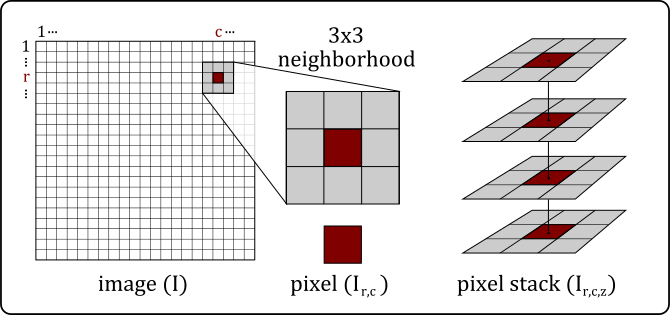
\includegraphics[width=4in]{FIGS/imaging/stack.pdf}
  {\singlespacing 
  \caption[ Pixel coordinate system.]
            { An image $I_{r,c}$ is a matrix of intensity values,
            with pixel coordinates
			given by row $r$ and column $c$. Analyses can
			be performed on single pixels, the entire image, image
			neighborhoods, or image stacks as shown. In the case of an image stack,
			$z$ refers to the image position within the stack. Note that $z$ need not
			refer to a height, as in the common z-stacks of confocal microscopy,
			but can also indicate different color
			channels or even entirely unrelated images. In effect, $z$
            is a ``height'' within the image stack that may not
            correspond to the physical height of an imaged within a sample.}
  \label{fig:imaging:stack}}
  \end{figure}


Each component of the image model in \ar{eq:imaging:simpleFullModel}
is a matrix of the same dimensions,
and each has distinct properties. The foreground components
of $F$ have completely idiosyncratic
values, both within and between images, as these
values depend on where cells are, what is
being stained, and what kinds of randomly-positioned
artifacts are present. Indeed, the
unknown behaviors of the foreground layers are 
what we typically aim to understand
via image analysis.


The background layers of $B$ are defined to
be more predictable, in that they are
unchanging by position within an image. The background should
be constant between images as well,
when identical experimental conditions
are used to obtain those images.
However, the total background
may change as a consequence of some experimental
perturbation. For example, some small
molecules used as drugs may fluoresce
and so add an additional background layer.
Finally, note that due to shading these
``flat'' background layers will appear
distorted in uncorrected images.
To clarify, then, I define background
layers as those that are constant across an image
in the absence of shading.


The detector layer $D$ has the simplest behavior, as it can be considered
constant regardless of the imaging and experimental conditions. ``Constant'' in this
case means that the value at any given pixel position $D_{r,c}$ does not change
over time or between images.
The values within an image, on the other hand, may vary
(see \ar{fig:imaging:properties}a).


The shading value $S$ is problematic for analysis in that it distorts the
$B$ and $F$ layers in non-trivial ways.
Like $D$, this layer also shows variation within an image.
The shading pattern caused by the objective lens
tends to show brighter fluorescence at image centers
and weaker fluorescence at the edges. However,
the presence of other components
in the light path, such as filters, can modify this shading pattern
(\ar{fig:imaging:properties}b) \cite{VandenDoel1998}.
Unlike $D$, the shading pattern can vary between
images as well, though in \ar{imaging:correction} I show that this variation
can be both predictable and correctable. $S$ distorts the $F$ and $B$ layers
multiplicatively, and can cause as
large as 1.5- to 2-fold intensity differences across an image
\cite{Bray2013}.




  \begin{figure}[!bt]
  \centering
  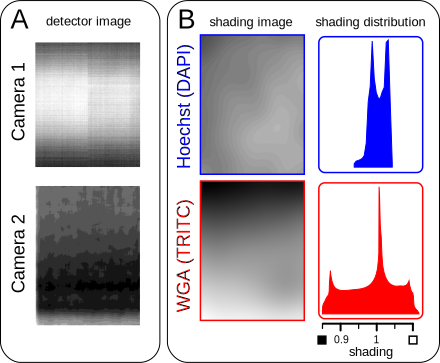
\includegraphics[width=4in]{FIGS/imaging/properties.pdf}
  {\singlespacing 
  \caption[ Example detector $D$ and shading $S$ patterns.]
            { Example within-image variation of the detector $D$
			and shading $S$ image components. \b{a}, Per-pixel
            averages of 10 detector images from
			two cameras are shown. Camera 1, Andor Zyla sCMOS 11-bit.
			Camera 2, Roper Scientific CoolSnap HQ2 CCD 14-bit.
            Intensities and
			images are scaled independently.
			\b{b}, Shading patterns from two optical channels. Uniformly-fluorescent
			background images were made with dissolved Hoechst or wheat
			germ agglutinin (WGA)-TRITC in the DAPI and TRITC optical channels. Note
			that each channel has a dramatically different shading pattern and overall
			degree of shading. Histograms show the all-pixel distributions
			of shading values, which are defined to have
			a median of one (a robust variant of $\E[S]\equiv 1$, defined in
			\ar{imaging:correction}).
			}
  \label{fig:imaging:properties}}
  \end{figure}


Finally, we are left with the noise term $\epsilon$. I use this
term specifically to capture measurement noise, not true biological
variability. The largest source of measurement
noise for modern fluorescence imaging
is probably due to the combination of two factors: the error in converting
photon counts to electrons, and the error introduced during transmission
of those electrons from the camera. Combined, this measurement error
introduces an intensity-dependent uncertainty in the total measured
intensity of the pixel $I_{r,c}$. In general, the relative error
decreases as a function of the square root of intensity \cite{Goldman2005}.


